
\documentclass[a4paper,12pt]{article}

\usepackage{graphicx} % Required for inserting images
\usepackage{amsmath,amssymb,amsfonts}
\usepackage{subcaption}
% -----------------------
% Package Imports
% -----------------------

% Set page margins
\usepackage[a4paper, top=1in, bottom=0.8in, left=1.1in, right=0.8in]{geometry}

% Use Times New Roman font
\usepackage{times}

% Add page numbering
\pagestyle{plain}

% Enable graphics inclusion
\usepackage{graphicx}
\usepackage{float}
% Enable code listings
\usepackage{listings}
\usepackage{xcolor} % For customizing code colors
\setlength{\parindent}{0pt}
\usepackage{physics}



\begin{document}
	\section{Experiment No. 9}
	
	\section{Experiment Title }
	Determination of Voltage Regulation of Single-Phase Transformer for different kinds of load.
	\section{Objective}
	
	The objectives of this lab are as follows:
	\begin{itemize}
		 \item To determine the voltage regulation of a single-phase transformer under different types of loads.
		\item To analyze the effects of resistive, inductive, and capacitive loads on the voltage regulation of the transformer.
		\item To understand the theoretical and practical behavior of voltage regulation for various load conditions.
	\end{itemize}
	
	\section{Theory}

\subsection{Voltage Regulation (V.R)}

Voltage Regulation (V.R) is a measure of the change in the secondary voltage of a transformer as the load varies, from no-load (NL) to full-load (FL). It is expressed as a percentage of the full-load voltage.  

The Voltage Regulation (V.R) is given by the formula:
\[
\text{V.R} = \frac{V_{\text{NL}} - V_{\text{FL}}}{V_{\text{FL}}} \times 100 \%
\]
Where:
\begin{enumerate}
	\item $V_{\text{NL}}$ is the no-load voltage (the voltage across the secondary when the transformer is not supplying any load),
	\item $V_{\text{FL}}$ is the full-load voltage (the voltage across the secondary when the transformer is supplying full-load current),
	\item $V_S$ is the secondary side voltage, which depends on the load and its nature.
\end{enumerate}

An alternate expression for voltage regulation can be written as:
\[
\text{V.R} = \frac{V_{\text{NL}} - V_S}{V_S}
\]
Where $V_S$ is the voltage at the secondary side under load conditions.

\subsection{Transformer Behavior Under Load Conditions}

The behavior of the transformer under different load conditions can be analyzed using the phasor equation:
\[
E_2 = V_S + I_S R_S + j I_S X_S
\]
Where:
\begin{enumerate}
	\item $E_2$: Secondary induced EMF (ideal voltage without losses),
	\item $V_S$: Secondary terminal voltage under load,
	\item $R_S$: Equivalent series resistance of the transformer,
	\item $X_S$: Equivalent series reactance of the transformer,
	\item $I_S$: Load current.
\end{enumerate}

\subsubsection*{Phasor Diagrams}
\begin{enumerate}
	\item \textbf{Capacitive Load:}  
	The current $I_S$ leads the voltage $V_S$. The phasor diagram shows that this interaction reduces the voltage drop, potentially causing a voltage rise, resulting in a \emph{negative} Voltage Regulation (V.R).
	
	\item \textbf{Inductive Load:}  
	The current $I_S$ lags the voltage $V_S$. The phasor diagram demonstrates significant voltage drops across $R_S$ and $X_S$, leading to a \emph{positive} Voltage Regulation (V.R).
	
	\item \textbf{Resistive Load:}  
	The current $I_S$ is in phase with the voltage $V_S$. The phasor diagram shows a moderate voltage drop, primarily due to $I_S R_S$.
\end{enumerate}

\subsection{Effect of Load Type on Voltage Regulation}

Different kinds of loads affect the voltage regulation of the transformer in distinct ways. These loads can be broadly classified as inductive, resistive, and capacitive loads.

\begin{enumerate}
	\item \textbf{Inductive Load:}  
	For an inductive load, the load current ($I_S$) lags the voltage, creating a lagging power factor. The voltage drop across the load is given by:
	\[
	\text{Voltage Drop} = I_S R_S + I_S X_S
	\]
	
\begin{figure}[H]
	\centering
	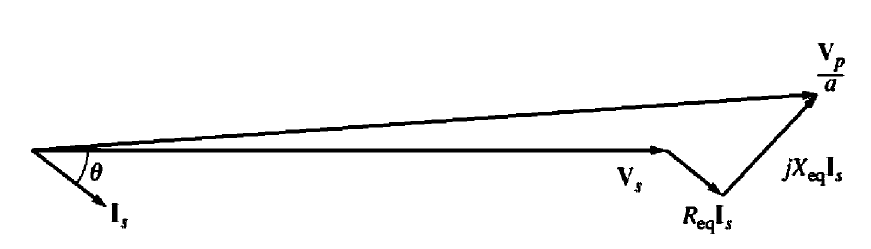
\includegraphics[width=0.6\linewidth]{Images/1.1}
	\caption{Phasor Diagram for Inductive Load}
	\label{fig:1}
\end{figure}
	As $I_S$ increases, the voltage drop increases, causing $V_S$ to decrease, resulting in positive Voltage Regulation.
	
	\item \textbf{Resistive Load:}  
	For a resistive load, the load current is in phase with the voltage, and the voltage drop is given by:
	\[
	\text{Voltage Drop} = I_S R_S
	\]
	
	\begin{figure}[H]
		\centering
		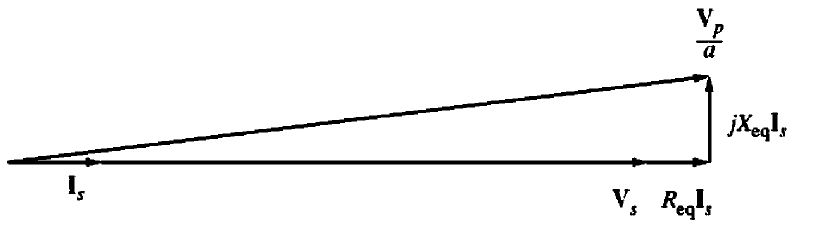
\includegraphics[width=0.6\linewidth]{Images/1.3}
		\caption{Phasor Diagram for Resistive Load}
		\label{fig:1}
	\end{figure}
	As $I_S$ increases, the voltage drop increases, causing $V_S$ to decrease. This results in positive Voltage Regulation, but the effect is smaller compared to an inductive load.
	
	\item \textbf{Capacitive Load:}  
	For a capacitive load, the current leads the voltage, resulting in a leading power factor. The voltage drop across the load is:
	\[
	\text{Voltage Drop} = I_S R_S - I_S X_C
	\]
	
	\begin{figure}[H]
		\centering
		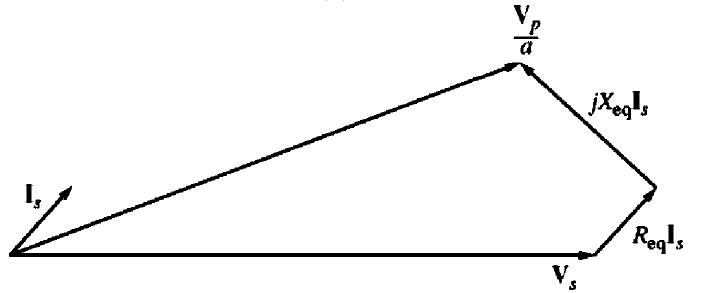
\includegraphics[width=0.6\linewidth]{Images/1.2}
		\caption{Phasor Diagram for Capacitive Load}
		\label{fig:1}
	\end{figure}
	As $I_S$ increases, the voltage drop decreases, causing $V_S$ to increase. This results in negative Voltage Regulation.
\end{enumerate}

	\begin{figure}[H]
	\centering
	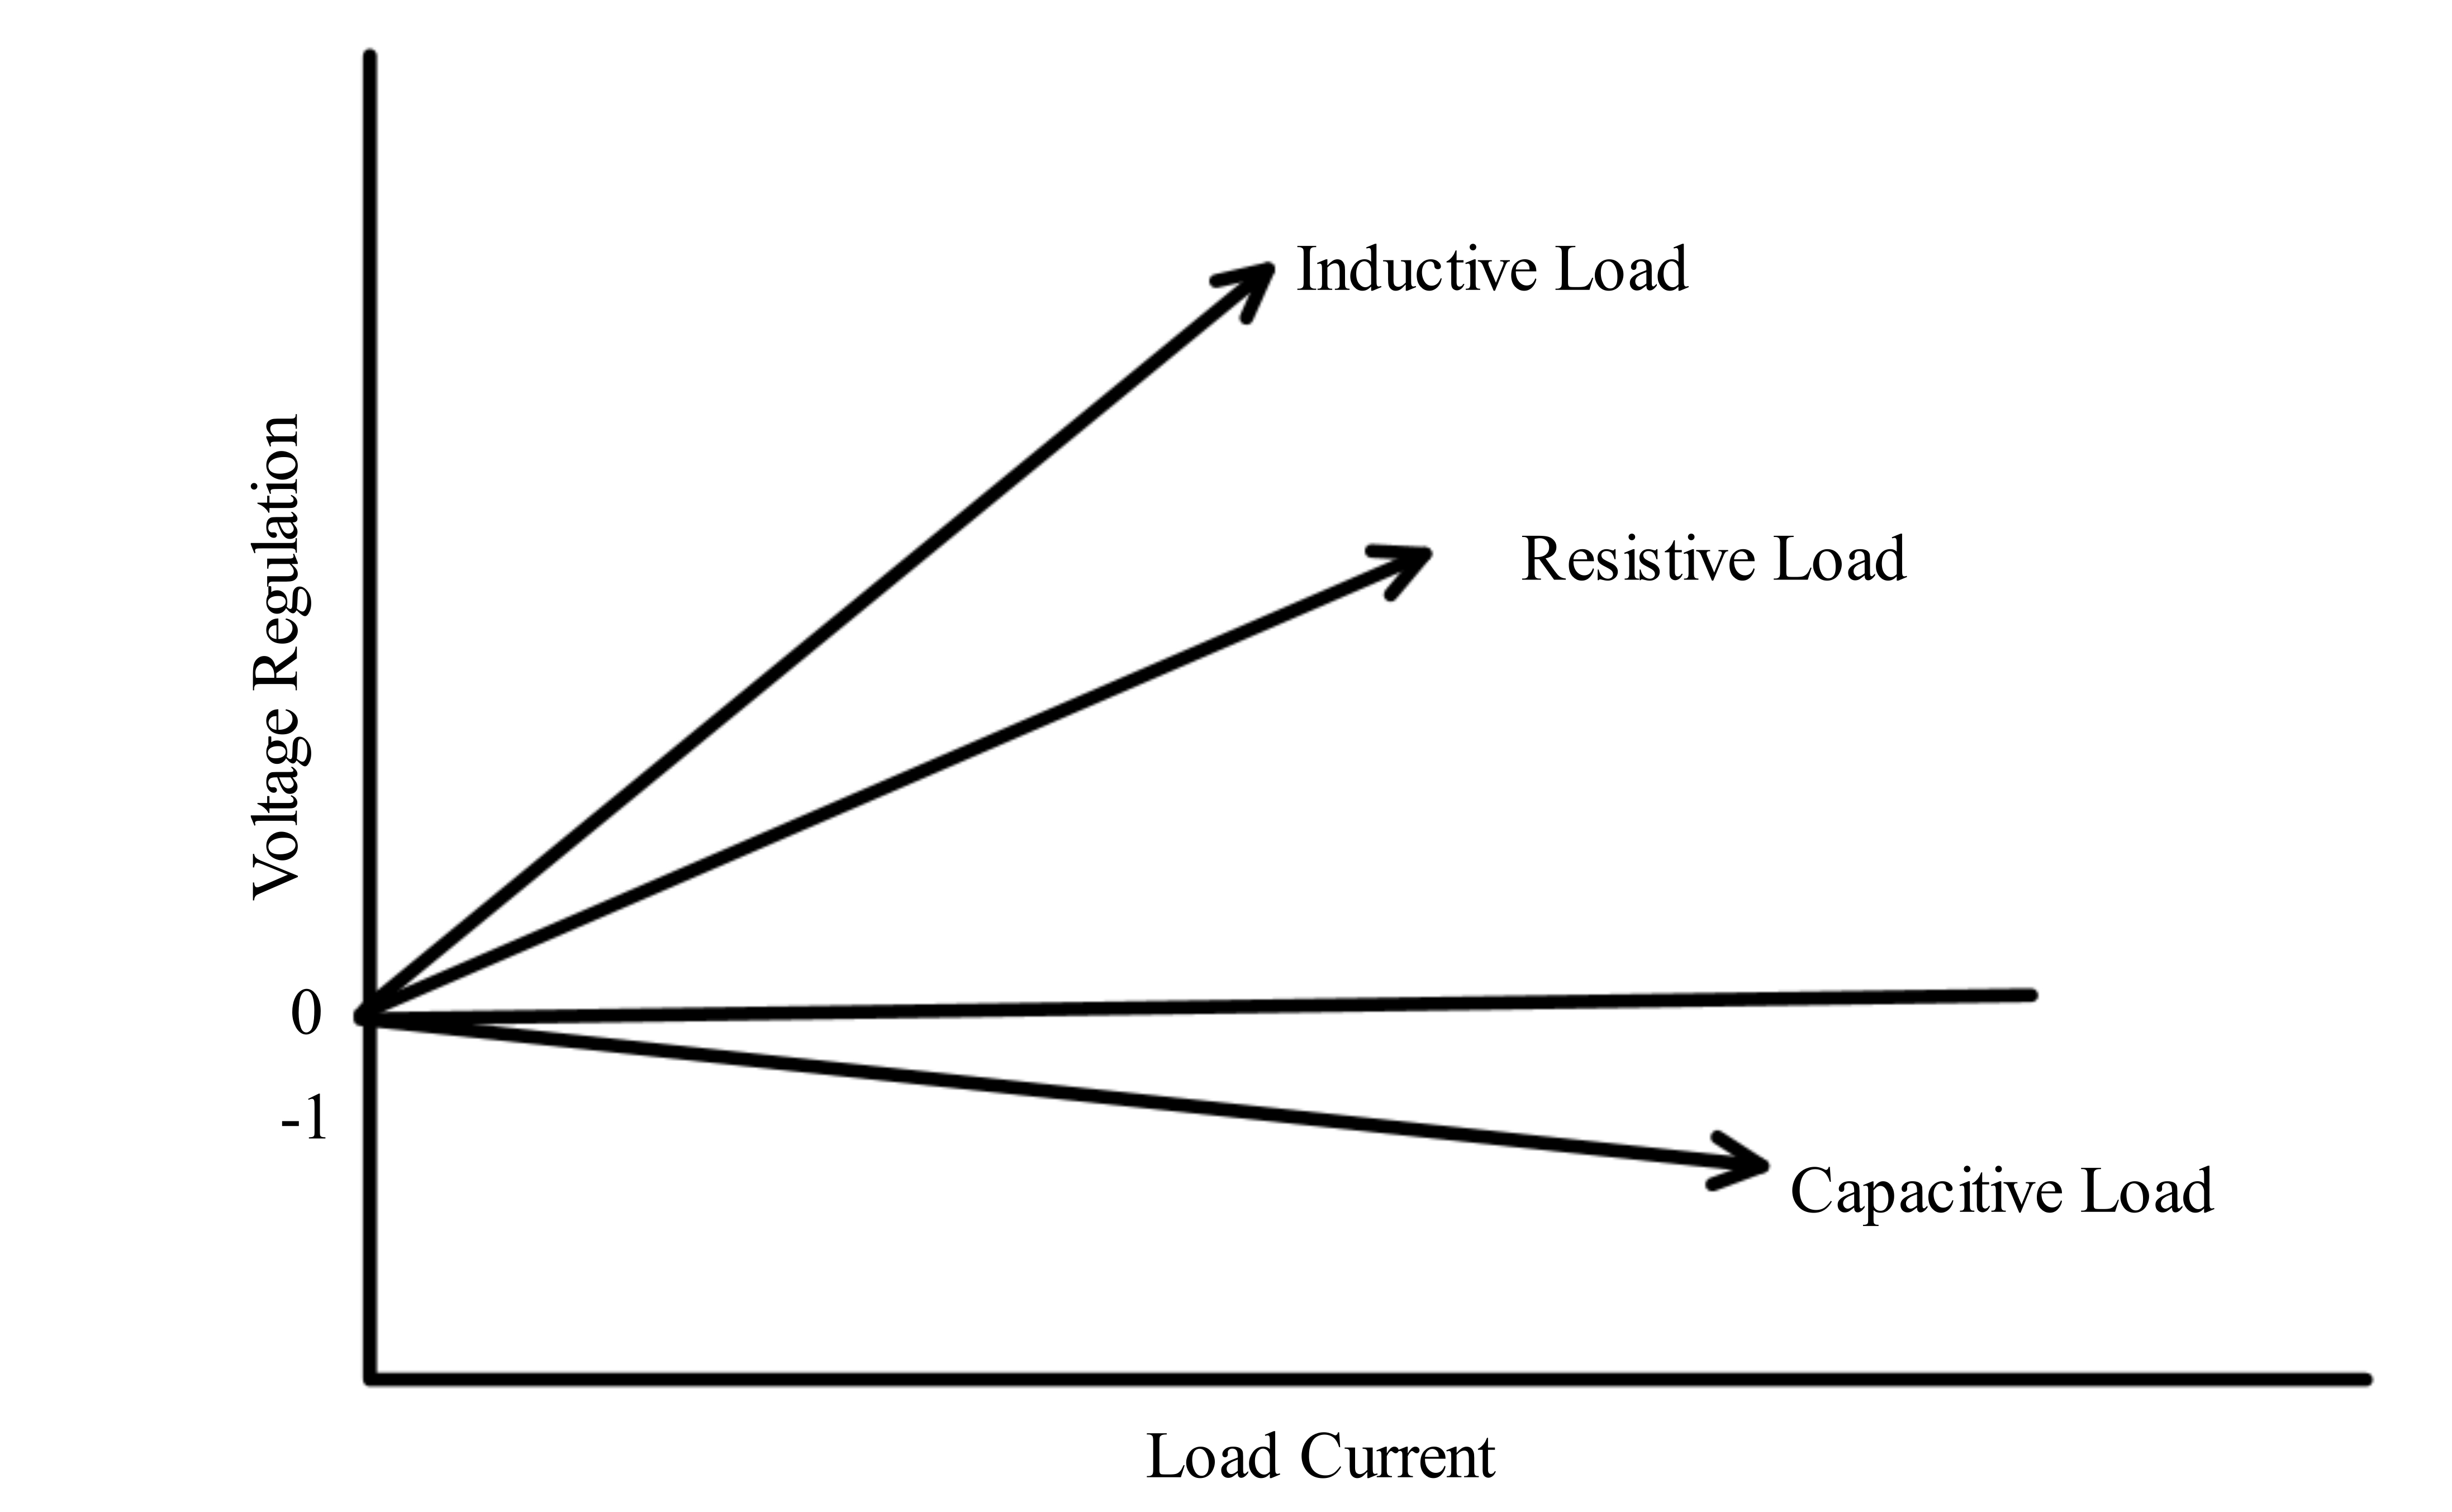
\includegraphics[width=0.71\linewidth]{Images/p}
	\caption{Voltage Regulation  vs Load Current }
	\label{fig:st}
\end{figure}







	\newpage
	\section{Required Apparatus}
	\begin{enumerate}
		\item \textbf{Transformer}
		\begin{enumerate}
			\item Power (\(P\)): 760 VA
			\item Primary Voltage (\(U_1\)): 230 V
			\item Secondary Voltage (\(U_2\)): 400 -- 230 V
			\item Frequency (\(f\)): 50 Hz
			\item Primary Current (\(i_1\)): 3.7 A
			\item Secondary Current (\(i_2\)): 1 -- 1.7 A
		\end{enumerate}

		\item \textbf{Resistive Loads (Mod. RL-1/EV: Ratings: 220-230V(DC)/380-400V(AC), 462W max):}
		\begin{enumerate}
			\item Load no. 1: Resistance: 2200 $\Omega$, Current: 0.1 A
			\item Load no. 2: Resistance: 1100 $\Omega$, Current: 0.2 A
			\item Load no. 3: Resistance: 550 $\Omega$, Current: 0.4 A
		\end{enumerate}
		
		\item \textbf{Capacitive Loads (Mod. CL-1/EV: Ratings: 220-230V/380-400V, 50Hz, 462VA max):}
		\begin{enumerate}
			\item Load no. 1: Capacitance: 1.4 $\mu$F, Current: 0.1 A, Reactance: 2200 $\Omega$
			\item Load no. 2: Capacitance: 2.9 $\mu$F, Current: 0.2 A, Reactance: 1100 $\Omega$
			\item Load no. 3: Capacitance: 5.8 $\mu$F, Current: 0.4 A, Reactance: 550 $\Omega$
		\end{enumerate}
		
		\item \textbf{Inductive Loads (Mod. IL-1/EV: Ratings: 220-230V/380-400V, 50Hz, 462VA max):}
		\begin{enumerate}
			\item Load no. 1: Current: 0.1 A, Reactance: 2200 $\Omega$
			\item Load no. 2: Current: 0.2 A, Reactance: 1100 $\Omega$
			\item Load no. 3: Current: 0.4 A, Reactance: 550 $\Omega$
		\end{enumerate}
		
		\item \textbf{Three Phase AC Meter:}
		\begin{enumerate}
			\item Ammeter: Current: 5 A max
			\item Voltmeter: Voltage: 500 V AC rms max
		\end{enumerate}
		
		\item \textbf{Three Phase AC Meter Display}
		\item \textbf{Connecting Wires}
	\end{enumerate}
	
	
	\section{Circuit Diagrram}
	
	
	\begin{figure}[H]
		\centering
		
			\centering
			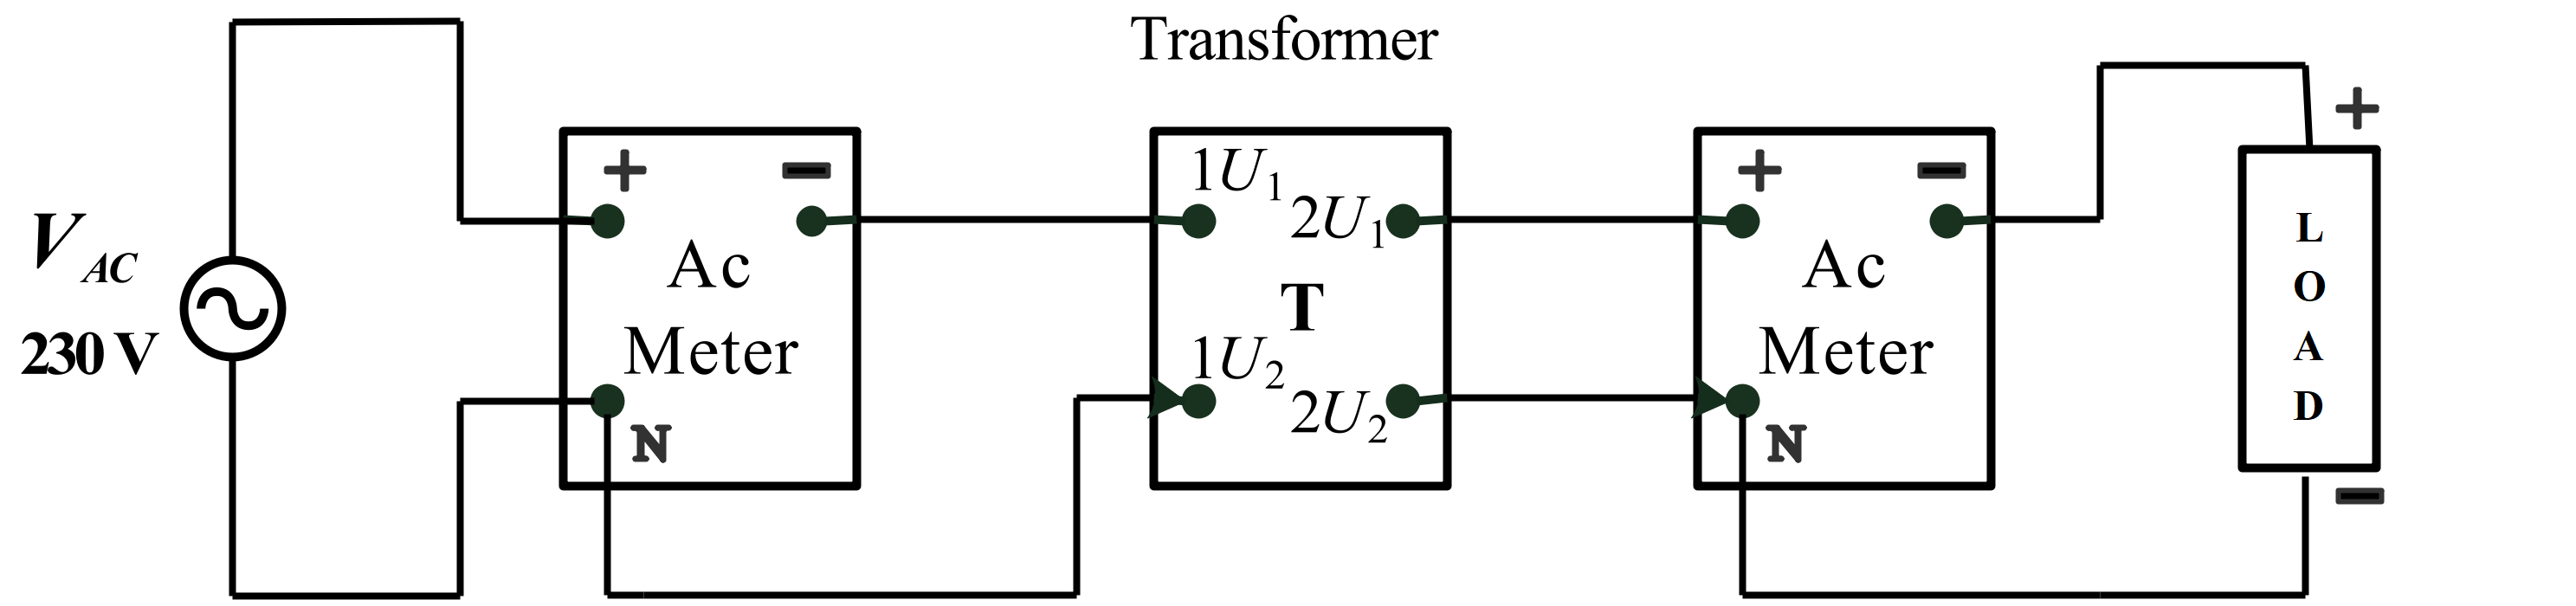
\includegraphics[width=1\linewidth]{Images/09}
			\caption{Connection of single phase transformer for different kinds of load.}
			\vspace{0.5cm}

	\end{figure}
	
	\newpage
	\section{Data Table}
	\begin{table}[H]
		\centering
		\caption{Voltage Regulations for Inductive Loads}
		\begin{tabular}{|c|c|c|c|c|}
			\hline
			\textbf{Sl. No.} & \begin{tabular}[c]{@{}c@{}}No Load Voltage\\  $E_2 (V)$\end{tabular} & \begin{tabular}[c]{@{}c@{}}Load Current, \\ $I_S(A) $\end{tabular} & \begin{tabular}[c]{@{}c@{}}Full Load Voltage, \\ $V_S(V)$\end{tabular} & \begin{tabular}[c]{@{}c@{}}Voltage Regulation \\$V_R (\%)$ \end{tabular} \\ \hline
			01.              & 424.6                                                                     & 0.000                                                              & 424.6                                                                  & 0                                                                   \\ \hline
			02.              & 424.6                                                                     & 0.174                                                              & 419.0                                                                  & 0.28                                                                \\ \hline
			03.              & 424.6                                                                     & 0.208                                                              & 423.7                                                                  & 0.47                                                                \\ \hline
			04.              & 424.6                                                                     & 0.69                                                               & 422.6                                                                  & 0.88                                                                \\ \hline
			05.              & 424.6                                                                     & 0.919                                                              & 417.1                                                                  & 1.34                                                                \\ \hline
			06.              & 424.6                                                                     & 1.104                                                              & 420.9                                                                  & 1.58                                                                \\ \hline
			07.              & 424.6                                                                     & 1.373                                                              & 418.0                                                                  & 1.8                                                                 \\ \hline
			08.              & 424.6                                                                     & 1.581                                                              & 416.8                                                                  & 1.87                                                                \\ \hline
		\end{tabular}
	\end{table}
	
	\begin{table}[H]
		\centering
		\caption{Voltage Regulations for Resistive Loads}
		\begin{tabular}{|c|c|c|c|c|}
			\hline
			\textbf{Sl. No.} & \begin{tabular}[c]{@{}c@{}}No Load Voltage\\     $E_2 (V)$\end{tabular} & \begin{tabular}[c]{@{}c@{}}Load Current, \\ $I_S(A) $\end{tabular} & \begin{tabular}[c]{@{}c@{}}Full Load Voltage, \\ $V_S(V)$\end{tabular} & \begin{tabular}[c]{@{}c@{}}Voltage Regulation \\ $V_R (\%)$\end{tabular} \\ \hline
			01.              & 424.6                                                                     & 0.000                                                              & 424.6                                                                  & 0                                                                   \\ \hline
			02.              & 424.6                                                                     & 0.188                                                              & 421.4                                                                  & 0.76                                                                \\ \hline
			03.              & 424.6                                                                     & 0.374                                                              & 417.5                                                                  & 1.94                                                                \\ \hline
			04.              & 424.6                                                                     & 0.737                                                              & 411.3                                                                  & 3.23                                                                \\ \hline
			05.              & 424.6                                                                     & 0.857                                                              & 415.0                                                                  & 3.81                                                                \\ \hline
			06.              & 424.6                                                                     & 0.915                                                              & 408.1                                                                  & 4.04                                                                \\ \hline
			07.              & 424.6                                                                     & 1.09                                                               & 404.5                                                                  & 4.97                                                                \\ \hline
			08.              & 424.6                                                                     & 1.26                                                               & 401.1                                                                  & 5.86                                                                \\ \hline
		\end{tabular}
	\end{table}
	
	
	\begin{table}[H]
		\centering
		\caption{Voltage Regulations for Capacitive Loads}
		\begin{tabular}{|c|c|c|c|c|}
			\hline
			\textbf{Sl. No.} & \begin{tabular}[c]{@{}c@{}}No Load Voltage\\  $E_2 (V)$\end{tabular} & \begin{tabular}[c]{@{}c@{}}Load Current, \\ $I_S(A) $\end{tabular} & \begin{tabular}[c]{@{}c@{}}Full Load Voltage, \\ $V_S(V)$\end{tabular} & \begin{tabular}[c]{@{}c@{}}Voltage Regulation \\ $V_R (\%)$\end{tabular} \\ \hline
			01.              & 424.6                                                                     & 0.00                                                               & 423.0                                                                  & 0.00                                                                 \\ \hline
			02.              & 424.6                                                                     & 0.204                                                              & 424.0                                                                  & -0.24                                                                \\ \hline
			03.              & 424.6                                                                     & 0.422                                                              & 424.4                                                                  & -0.33                                                                \\ \hline
			04.              & 424.6                                                                     & 0.619                                                              & 424.7                                                                  & -0.40                                                                \\ \hline
			05.              & 424.6                                                                     & 0.791                                                              & 424.8                                                                  & -0.42                                                                \\ \hline
			06.              & 424.6                                                                     & 0.984                                                              & 424.9                                                                  & -0.45                                                                \\ \hline
			07.              & 424.6                                                                     & 1.195                                                              & 425.1                                                                  & -0.49                                                                \\ \hline
			08.              & 424.6                                                                     & 1.402                                                              & 425.3                                                                  & -0.54                                                                \\ \hline
		\end{tabular}
	\end{table}
	
	\section{Graph}
	
	\begin{figure}[H]
		\centering
		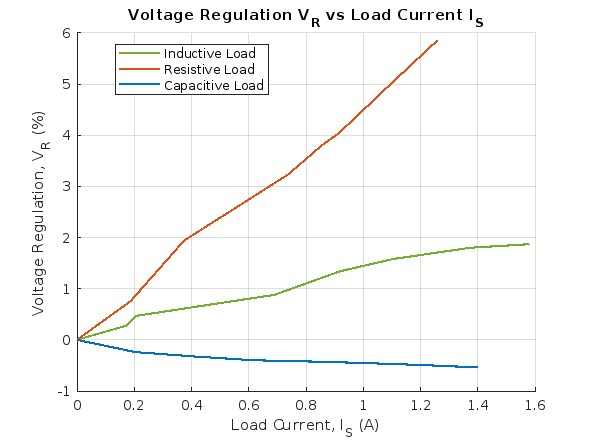
\includegraphics[width=1\linewidth]{Images/exp9}
		\caption{Voltage Regulation $V_R$ vs Load Current $I_S$}
		\label{fig:st}
	\end{figure}

	\section{Discussion}
	
	The experiment was conducted to determine the voltage regulation of a single-phase transformer for different types of loads.\\ It was demonstrated through the experiment that the voltage regulation of a single-phase transformer was significantly affected by the type of load connected. Theoretically, the voltage regulation for inductive loads should have been greater than for resistive loads. However, positive voltage regulation was observed to be the highest with resistive loads, while moderate voltage regulation was exhibited under inductive loads due to the combined effects of magnitude and phase changes. Negative voltage regulation, indicating a voltage rise, was recorded for capacitive loads. These variations were found to be essential for understanding transformer behavior and ensuring their performance under different load conditions.
	
	
\end{document}
